
\documentclass[12pt, a4paper, titlepage]{article}

% Soporte multilenguaje para LaTeX.
\usepackage[spanish]{babel}

% Interfaz flexible para definir las dimensiones del documento
\usepackage[a4paper, top=2.5cm, bottom=2.5cm, left=2.5cm, right=2.5cm]{geometry} 

% Aceptar diferentes tipos de codificación de caracteres de entrada (en este caso usamos la codificación Unicode UTF-8)
\usepackage[utf8]{inputenc} 

% Soporte aumentado para gráficos 
\usepackage{graphicx}
%\usepackage[pdftex]{graphicx}

% Partir correctamente tablas
\usepackage{longtable}

% Escribir enumerados
\usepackage{enumerate}

% Cabeceras y pies de página
\usepackage{fancyhdr}
%\pagestyle{empty}
%\newcommand\fancysection[2]{
%	\pagebreak
%	\section{#1. #2}
%	\renewcommand\leftmark{#1}
%	\renewcommand\rightmark{#2}
%}
%\fancyhead[HC]{}
%\fancyhead[HL]{\slshape \MakeUppercase{\leftmark}}
%\fancyhead[HR]{\slshape \MakeUppercase{\rightmark}}
%\setlength{\headheight}{15pt}

% Índice con links
\usepackage[colorlinks=true,linkcolor=blue]{hyperref}

% Otros comandos
\newcommand\tittleditem[1]{\item \textbf{#1}\\}

% Código
\usepackage{listings}
\usepackage{color}

\definecolor{dkgreen}{rgb}{0,0.6,0}
\definecolor{gray}{rgb}{0.5,0.5,0.5}
\definecolor{mauve}{rgb}{0.58,0,0.82}

% descomenta "numbers=none" para quitar los numeros de línea
% y copy-pastear código mas comodamente
\lstset{
  frame=single,
  language=c,
  aboveskip=3mm,
  belowskip=3mm,
  showstringspaces=false,
  columns=flexible,
  basicstyle={\small\ttfamily},
  numbers=left,
  %numbers=none,
  stepnumber=1,
  numberstyle=\tiny\color{gray},
  keywordstyle=\color{blue},
  commentstyle=\color{dkgreen},
  stringstyle=\color{mauve},
  breaklines=true,
  breakatwhitespace=true,
  tabsize=3,
  inputencoding=utf8,
  literate={ä}{{\"a}}1
           {ë}{{\"e}}1
           {ï}{{\"i}}1
           {ö}{{\"o}}1
           {ü}{{\"u}}1
           {Ä}{{\"A}}1
           {Ë}{{\"E}}1
           {Ï}{{\"I}}1
           {Ö}{{\"O}}1
           {Ü}{{\"U}}1
           {á}{{\'a}}1
           {é}{{\'e}}1
           {í}{{\'i}}1
           {ó}{{\'o}}1
           {ú}{{\'u}}1
           {Á}{{\'A}}1
           {É}{{\'E}}1
           {Í}{{\'I}}1
           {Ó}{{\'O}}1
           {Ú}{{\'U}}1
           {ñ}{{\~n}}1
           {Ñ}{{\~N}}1
}

\begin{document}

\begin{titlepage}

\begin{center}


\includegraphics[width=13cm]{./img/logo_UDC.png}
\vspace*{0.5in}

FACULTAD DE INFORMÁTICA DE LA CORUÑA\\
\vspace*{2.5in}

\begin{Large}
\textbf{Foro simple en Pro*C} \\
\end{Large}
\vspace*{0.1in}

\begin{large}
\textit{Trabajo tutelado de Bases de Datos Avanzadas} \\
\end{large}
\vspace*{0.4in}

\begin{large}
Curso 2013-2014
\end{large}
\vspace*{3.4in}


\rule{80mm}{0.1mm}\\
\vspace*{0.25in}

\begin{large}
\textbf{Alejandro Fortes Lopes}\\
\textbf{Elías Grande Cásedas}\\
\end{large}

\end{center}

\end{titlepage}

\tableofcontents

\pagestyle{fancy}

\pagebreak
\section{Diseño conceptual}

\subsection{Descripción del dominio}

El dominio que hemos escogido para este trabajo es un foro de discusión formado por diferentes subforos, hilos y entradas y con una gestión muy básica de usuarios.
\paragraph{}
La aplicación se conectará directamente a la base de datos y le permitirá al usuario visualizar las discusiones, y realizar diferentes operaciones (edición y borrado) en función de los permisos que posea.

\subsection{Diagrama Entidad-Relación}

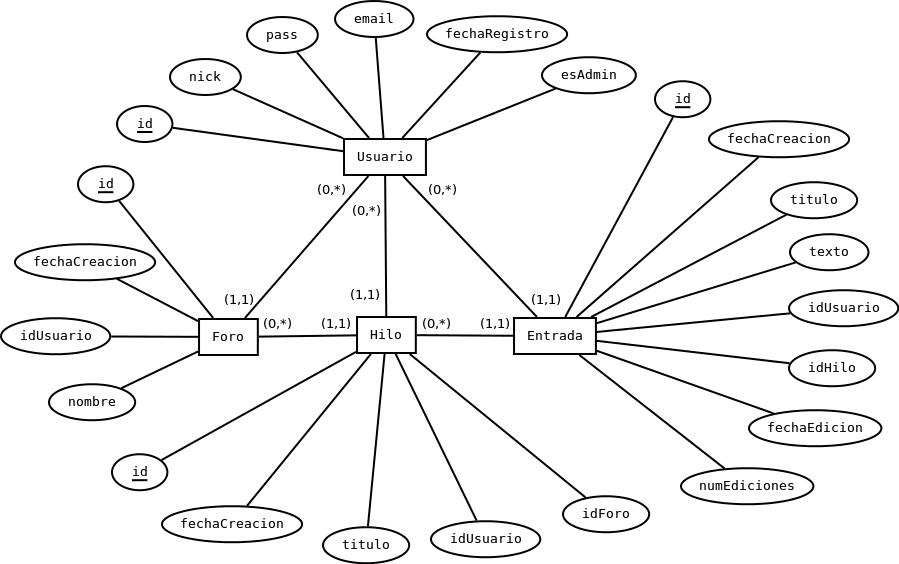
\includegraphics[width=15cm]{./img/er.png}

\subsection{Diccionario de datos}

\subsubsection{Entidades}

\begin{longtable}{|p{3cm}|p{4cm}|p{6cm}|}
	\hline
	\textbf{Identificador} & \textbf{Descripción} & \textbf{Características} \\ \hline
	\endhead
	Usuario & Individuo con permisos de acceso al foro & Puede leer foros, hilos, entradas, también crearlos y, si es el autor o admin, editarlos y borrarlos. \\ \hline
	Foro & Sala de discusión organizada en hilos temáticos. & Contiene una lista de hilos en los que se discute cada tema mediante mensajes. \\ \hline
	Hilo & Conjunto de mensajes de una discusión concreta. & Está formado por una lista de entradas. \\ \hline
	Entrada & Cada uno de los mensajes de un hilo. & Son creados por usuarios registrados, y solo pueden ser eliminados o editados por el creador o un administrador (también puede ser eliminado como parte de un hilo, borrado en cascada). \\ \hline
\end{longtable}

\subsubsection{Atributos de Usuario}

\begin{tabular}{|p{3cm}|p{2cm}|p{4cm}|p{4cm}|}
	\hline
	\textbf{Identificador} & \textbf{Tipo} & \textbf{Descripción} & \textbf{Características} \\ \hline
	id & int & Identificador. & Clave primaria. \\ \hline
	nick & varchar(20) & Nombre de usuario. & No puede ser nulo ni repetir valores. \\ \hline
	pass & varchar(32) & Contraseña de acceso. & No puede ser nulo. \\ \hline
	email & varchar(45) & Correo electrónico. & No puede ser nulo ni repetir valores. \\ \hline
	fechaRegistro & date & Fecha de registro. & No puede ser nula. \\ \hline
	esAdmin & char(1) & Indica si es administrador o no. & Debe ser `S' (si) o `N' (no). \\ \hline
\end{tabular}

\subsubsection{Atributos de Foro}

\begin{tabular}{|p{3cm}|p{2cm}|p{4cm}|p{4cm}|}
	\hline
	\textbf{Identificador} & \textbf{Tipo} & \textbf{Descripción} & \textbf{Características} \\ \hline
	id & int & Identificador. & Clave primaria. \\ 
	\hline
	fechaCreacion & date & Fecha de creación. & No puede ser nula. \\ \hline
	nombre & varchar(45) & Nombre descriptivo. & No puede ser nulo. \\ \hline
	idUsuario & int & Usuario creador del foro. & No puede ser nulo. Clave foránea hacia Usuario. \\ \hline
\end{tabular}

\subsubsection{Atributos de Hilo}

\begin{tabular}{|p{3cm}|p{2cm}|p{4cm}|p{4cm}|}
	\hline
	\textbf{Identificador} & \textbf{Tipo} & \textbf{Descripción} & \textbf{Características} \\ \hline
	id & int & Identificador. & Clave primaria. \\ 
	\hline
	fechaCreacion & date & Fecha de creación. & No puede ser nula. \\ \hline
	titulo & varchar(45) & Nombre descriptivo. & No puede ser nulo \\
	\hline	
	idUsuario & int & Usuario creador del hilo. & No puede ser nulo. Clave foránea hacia Usuario. \\ \hline
	idForo & int & Foro al que pertenece. & No puede ser nulo. Clave foránea hacia Foro.\\ 
	\hline
\end{tabular}


\subsubsection{Atributos de Entrada}

\begin{tabular}{|p{3cm}|p{2,5cm}|p{4cm}|p{4cm}|}
	\hline
	\textbf{Identificador} & \textbf{Tipo} & \textbf{Descripción} & \textbf{Características} \\ \hline
	id & int & Identificador. & Clave primaria. \\ 
	\hline
	fechaCreacion & date & Fecha de creación. & No puede ser nula. \\ \hline
	titulo & varchar(45) & Nombre descriptivo & No puede ser nulo. \\
	\hline	
	texto & varchar(1000) & Representa el contenido del mensaje & No puede ser nulo. \\
	\hline
	fechaEdición & date & Fecha de la última edición de la entrada. & Se inicializa a nulo. \\
	\hline
	numEdición & int & Número de veces que se ha editado la entrada. & Por defecto 0. \\
	\hline
	idUsuario & int & Usuario creador de la entrada. & No puede ser nulo. Clave foránea hacia Usuario. \\ 
	\hline
	idHilo & int & Hilo al que pertenece. & No puede ser nulo. Clave foránea hacia Usuario. \\ 
	\hline
\end{tabular}

\pagebreak
\section{Diseño lógico}

\subsection{Modelo relacional}

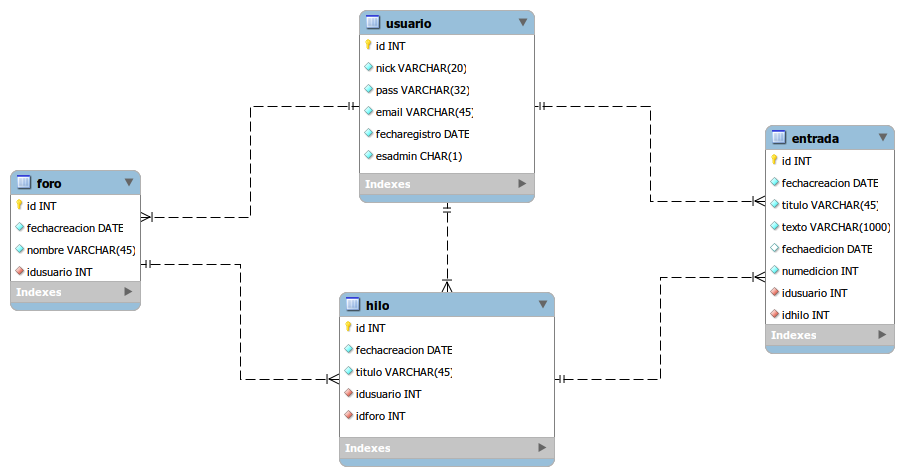
\includegraphics[width=15cm]{./img/relacional.png}

En modelo relacional se corresponde a la perfección (salvo algún detalle de nombrado) con lo ya descrito en el diccionario de datos del modelo conceptual.


\end{document}
